\documentclass{article}
\usepackage{amsmath}
\usepackage{setspace}

\usepackage{graphicx}
\graphicspath{{images/}}
\usepackage{wrapfig}
\usepackage{comment}
\usepackage{listings}
\usepackage{xcolor}
\usepackage{float}
%\usepackage[style=numeric]{biblatex}
%\addbibresource{fish.bib}
\usepackage{comment}

\definecolor{codegreen}{rgb}{0,0.6,0}
\definecolor{codegray}{rgb}{0.5,0.5,0.5}
\definecolor{codepurple}{rgb}{0.58,0,0.82}
\definecolor{backcolour}{rgb}{0.95,0.95,0.92}
 
\lstdefinestyle{mystyle}{
    backgroundcolor=\color{backcolour},
    commentstyle=\color{codegreen},
    keywordstyle=\color{magenta},
    numberstyle=\tiny\color{codegray},
    stringstyle=\color{codepurple},
    basicstyle=\fontsize{10}{12}\ttfamily,
    breakatwhitespace=false,
    breaklines=true,
    %breaklines=false,
    captionpos=b,
    keepspaces=true,
    numbers=left,
    numbersep=5pt,
    showspaces=false,
    showstringspaces=false,
    showtabs=false,
    tabsize=2
}
 
\lstset{style=mystyle}

%\usepackage[letter,margin=1.5in]{geometry}
%\addtolength{\rightmargin}{-0.5in}
%\addtolength{\textwidth}{0.5in}
%\addtolength{\oddsidemargin}{-.875in}
%\addtolength{\evensidemargin}{-.875in}
%\addtolength{\textheight}{1.75in}

\makeatletter
\renewcommand\section{\clearpage\newpage\@startsection {section}{1}{\z@}%
	{-3.5ex \@plus -1ex \@minus -.2ex}%
	{2.3ex \@plus.2ex}%
	{\normalfont\Large\bfseries}}
\makeatother

\newlength{\mylen}
\definecolor{darkRed}{rgb}{0.6,0,0}
\newcommand{\yf}[1]{{\color{darkRed}{#1}}}

\begin{document}

%==========================================================================
%==========================================================================
% Title pages.

%\begin{comment}
\newcommand{\mytitle}{Automatic Fish Tracking: 
Keeping Track of Who’s Who}
\newcommand{\myauthor}{Ari Spraggins}

\newcommand{\myskip}{\vspace{0.5in}}
\newcommand{\layouttitle}[1]{{\bf\large\MakeUppercase{#1}}}
\setlength{\parindent}{0em}
\doublespace
\pagenumbering{roman}
\thispagestyle{empty}

\begin{center}

	\vspace{4in} 
	\layouttitle{\mytitle} \\ by \\ \myauthor
	
	\vspace{1in}
	A Thesis Submitted to the Faculty of \\
	The Wilkes Honors College \\
	in Partial Fulfillment of the Requirements for the Degree of \\
	Bachelor of Science in Liberal Arts and Sciences \\
	with a Concentration in Physics \\ 
	\vspace{1in} 
	Wilkes Honors College of \\
	Florida Atlantic University \\
	Jupiter, Florida \\
	May \number\year

\end{center}

\newpage

%==========================================================================

\vspace{4in}
\begin{center}
	\layouttitle{\mytitle} \\
	by \\
	\myauthor
\end{center}

\singlespace
\vspace{1in}
This thesis was prepared under the direction of the candidate's thesis advisor, Dr. Yaouen Fily, and has been approved by the members of their supervisory committee. It was submitted to the faculty of the Harriet L. Wilkes Honors College and was accepted in partial fulfillment of the requirements for the degree of Bachelor of Science in Liberal Arts and Sciences.

\vspace{1in}
SUPERVISORY COMMITTEE:

\newcommand{\myrule}{\vspace{0.5in}\rule{4in}{0.5pt} \\}

\myrule
Dr. Yaouen Fily 

\myrule 
{}[second reader]

\myrule
Dean Justin Perry, Harriet L. Wilkes Honors College 

\myrule
Date

\newpage

%==========================================================================

%\begin{center}
%	\layouttitle{Acknowledgements}
%\end{center}
%\section*{Acknowledgements}
%%\addcontentsline{toc}{section}{Acknowledgements}
%
%\myskip
%Some acknowledgements.
%
%\newpage

%==========================================================================

%\begin{center}
%	\layouttitle{Abstract}
%\end{center}
\section*{Abstract}
\addcontentsline{toc}{section}{Abstract}

\myskip
\renewcommand{\arraystretch}{1.5}
\begin{tabular}{@{}l@{\hspace{3ex}}l}
	Author: & \myauthor \\
	Title: & \mytitle \\
	Institution: & Harriet L. Wilkes Honors College, Florida Atlantic University \\
	Thesis Advisor: & Dr. Yaouen Fily \\
	Degree: & Bachelor of Science in Liberal Arts and Sciences \\
	Concentration: & Physics \\
	Year: & \the\year
\end{tabular}

\myskip
\doublespace
%\end{comment}
Automatic video tracking has had a major impact on animal behavior studies. One of the challenges of this technique is keeping track of the identities of the fish, especially when they swim together and exchange positions. In this project we use the python programming language to address this problem for groups of fish. The video data comes from schooling assays performed at FAU's Cavefish Trilab (Dr. Keene, Dr. Duboue, and Dr. Kowalko). The method is inspired by the idTracker animal tracking software: we track patterns of brigthness as a visual identifier of each fish which we then use to detect when the fish swap places.
\newpage

%\begin{comment}
%==========================================================================

\tableofcontents

%\listoftables

\listoffigures

\newpage

%==========================================================================
%\end{comment}

\setlength{\parindent}{1em}
\pagenumbering{arabic}
%\singlespace

%==========================================================================
%==========================================================================
% Thesis proper.


\section{Introduction}

\subsection{Tracking Animal Behaviour}
While visually pleasing, schooling is a rather challenging topic that has long intrigued animal scientists. In order to quantify the animals' behavior, a vast quantity of positional data is needed; more than can be collected by hand. Advances in computer vision technology now make this type of data accessible through computerized video-tracking. Beyond schooling, this allows to quantify a wide variety of behaviors in a very accurate manner.

%talk about how interested in how schooling came to be? Schooling dynamics of related groups can provide insight in to how groups evolved. Now talk about trilab studying species that has variants that both do and don't school that are similar.
This thesis focuses on tracking the motion of Mexican Tetra fish (\textit{Astyanax mexicanus}). One of the quirks of the Mexican Tetra species is that some of its populations have been living in underground caves for about a million years. There, they have evolved a number of behavioral differences with the populations living on the surface, including the loss of schooling: whereas surface populations of \emph{A. mexicanus} school, cave-adapted ones do not~\cite{kowalko_utilizing_2020}. 

The data used in this thesis comes from experiments performed on campus in the labs of Dr. Keene, Dr. Dubou\'e, and Dr. Kowalko, collectively known as the Cavefish Trilab. The tracking software that the project aims to improve on was developed by Dr. Fily's group for the Cavefish Trilab~\cite{patch_kinematic_2020, patch_patchmemorycvtracer_2020}. The current version of that software has trouble maintaining the identities of the fish throughout an experiment. The purpose of this work is to fix that issue.

\subsection{Nature of the problem}

Before discussing how to maintain the identity of the fish as we track them, we must first talk a little about how the software locates them. Throughout the thesis {\bf we focus on two-fish experiments}. 
In each frame of the video, the software identifies regions that are darker than their surrounding. After filtering out dark regions whose size of aspect ratio is inconsistent with a fish, each remaining dark spot is interpreted as a fish. This works well for determining the positions of the fish at any given moment, but the identities of the fish can swap (fish 1 becomes fish 2 and vice versa) at any time.

\begin{figure}[H]
	\centering
	\setlength{\mylen}{0.32\linewidth}
	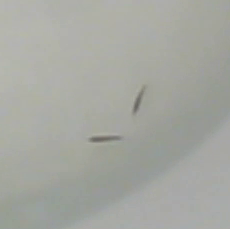
\includegraphics[height=\mylen]{140cropped}%
	\hspace{0.01\linewidth}%
	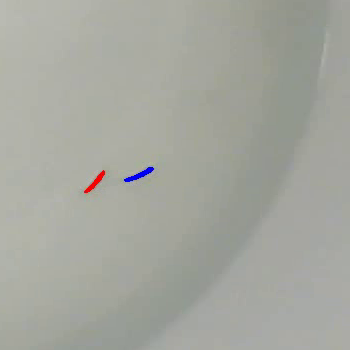
\includegraphics[height=\mylen]{simple-swap1}%
	\hspace{0.01\linewidth}%
	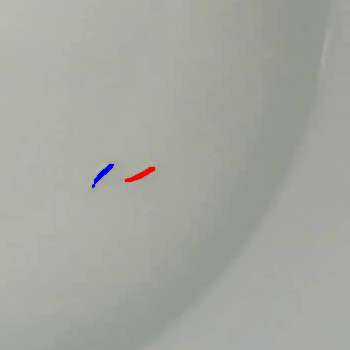
\includegraphics[height=\mylen]{simple-swap2}
	\caption{\emph{Left}: Close-up of two fish in their tank. The tank is made of white plastic. Each fish appears as a dark spot. \emph{Middle and Right}: Two consecutive frames of a two-fish video. Fish 1 is highlighted in blue. Fish 2 is highlighted in red. Basic dark spot detection makes no attempt to maintain the color ID of the fish, i.e., the colors can swap at any time.}
	\label{fig:fish}
\end{figure}

Many of those identity swaps can be fixed by analyzing the distance traveled by each fish. The videos are shot at 30 frames per second, so fish do not move much from one frame to the next. Therefore, the correct ID of a dark spot can often be obtained by matching each dark spot in the frame to the closest dark spot in the previous frame.

%\begin{figure}[H]
%	\centering
%	\setlength{\mylen}{0.32\linewidth}
%	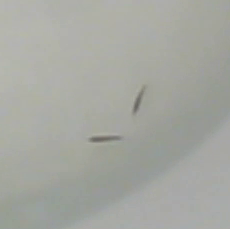
\includegraphics[height=\mylen]{140cropped}%
%	\caption{Left: Close-up of two fish in their tank. The tank is made of white plastic. Each fish appears as a dark spot. Middle and Right: Two consecutive frames of a two-fish video. Fish 1 is highlighted in blue. Fish 2 is highlighted in red. Basic dark spot detection makes no attempt to maintain the color ID of the fish, i.e., the colors can swap at any time.}
%	\label{fig:fish}
%\end{figure}

However, this does not always work. Issues occur in two scenarios. : when the fish get close enough that the program thinks there is only one fish (figure~\ref{fig:overlap-event}), and when the fish move fast enough that they are closer to the other's previous position then their previous position. The first of these issues is the easier of the two to check, since it is fairly trivial to check for regions in which only one fish is reported (please see Appendix~\ref{appendix1}). While it is easy enough to check for the first of these issues, the second is a little tougher. To check for errors in these cases, the distance of each fish from its previous position must be compared to the distance from each fish to the other fishes previous position (Appendix~\ref{app:swapStatus}). If the software mistakes the positions of the fish, which we will refer to as a swap, it will look like the fish traveled longer than it should have.



If the fish are near each other and moving fast, then a fish may closer to the previous position of another fish than to its own previous position. In that case, the distance-based method will swap the two fish's identities. 
If the fish are even closer, or if one is over or under another, the algorithm may only detect a single large dark spot. We call this an overlap event. An example is shown in Figure~\ref{fig:overlap-event}. Eventually, the fish separate and the algorithm detects them as distinct dark spots again, but the fish identities are lost in the process and 
\begin{figure}[H]
	\centering
	\setlength{\mylen}{0.32\linewidth}
	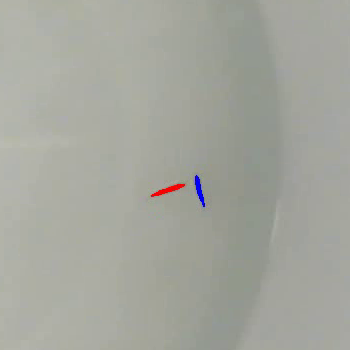
\includegraphics[height=\mylen]{overlap-event1}%
	\hspace{0.01\linewidth}%
	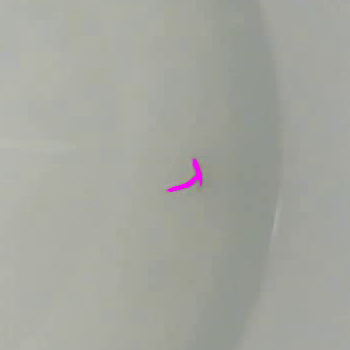
\includegraphics[height=\mylen]{overlap-event2}%
	\hspace{0.01\linewidth}%
	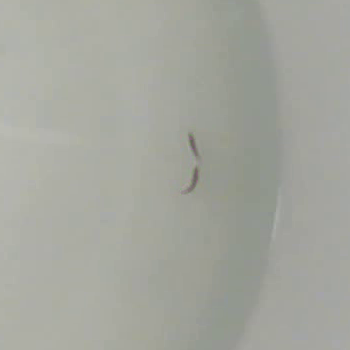
\includegraphics[height=\mylen]{overlap-event3}
	\caption{Overlap event. 
		\emph{Left}: Before the overlap, fish 1 (blue) is on the right and fish 2 (red) is on the left. 
		\emph{Middle}: During the overlap, the dark spot detection algorithm only detects one object (purple). The identities of the fish are meaningless because the algorithm thinks they are at the exact same place. 
		\emph{Right}: After the overlap, the fish identities cannot be recovered by analyzing the distance traveled.}
	\label{fig:overlap-event}
\end{figure}



\subsection{Previous work}

%reference idtracker/trex for how to talk about previous works, start broader, start with program that isn't able to auto unswap, recently programs came around that tried to automate this, paragraph about trex?
%\cite all of the papers, cite some of the things that are in the front of the papers, cite papers on mexican cavefish
%several haveemerged recently, all have upsides and downsides, ideal program depends on usecase

Video-tracking software designed with multi-animal experiments in mind typically handle the first type of identity swap described above -- the ones that are fixable by analyzing the distance traveled between frames. Swaps caused by overlap situations are trickier. Some older video-tracking software offer the possibility to fix the animals' tracks by hand after running the automatic tracking. A popular example is the commercial video-tracking software Ethovision, made by Noldus. The downside of this approach is that it is slower. In some cases, fixing all identity swaps by hand can become the most time-consuming part of the project. 

In recent years, several new software have come out to address this issue using various strategies.

The one this thesis is most heavily inspired from is idTracker~\cite{perez-escudero_idtracker_2014}. The idea is that each fish has a unique pattern of brighter and darker spots on its body, which can be used to recognize the fish even after loosing its track for a while. To quantify those patterns, the program measures spatial brightness correlations over each fish's body and compare them with previous frames to decide whether an identity swap has occurred. A more recent version of this software, known as idTracker.ai, uses machine learning methods to perform this task.

More recently, TRex~\cite{walter_trex_2021} provides a similar workflow but uses deep-learning methods to identify a visual pattern unique to each fish.

DeepLabCut~\cite{mathis_deeplabcut_2018} also uses deep-learning methods, however it solves a more ambitious problem: tracking multiple points of interest on each animal in order to quantify their posture as well as their position. The trade-off here is that the user has to manually identify the points of interest in several frames across the video, which is a bit more labor-intensive.


\subsection{Roadmap}

The goal of this project is to draw from the original idTracker approach to help fix identity swaps in a pre-existing video-tracking code designed for use in Cavefish Trilab: cvtracer~\cite{patch_kinematic_2020, patch_patchmemorycvtracer_2020}.

\yf{[Give a brief overview what's covered in each section of the thesis]}



%\begin{figure}[H]
%	\centering
%	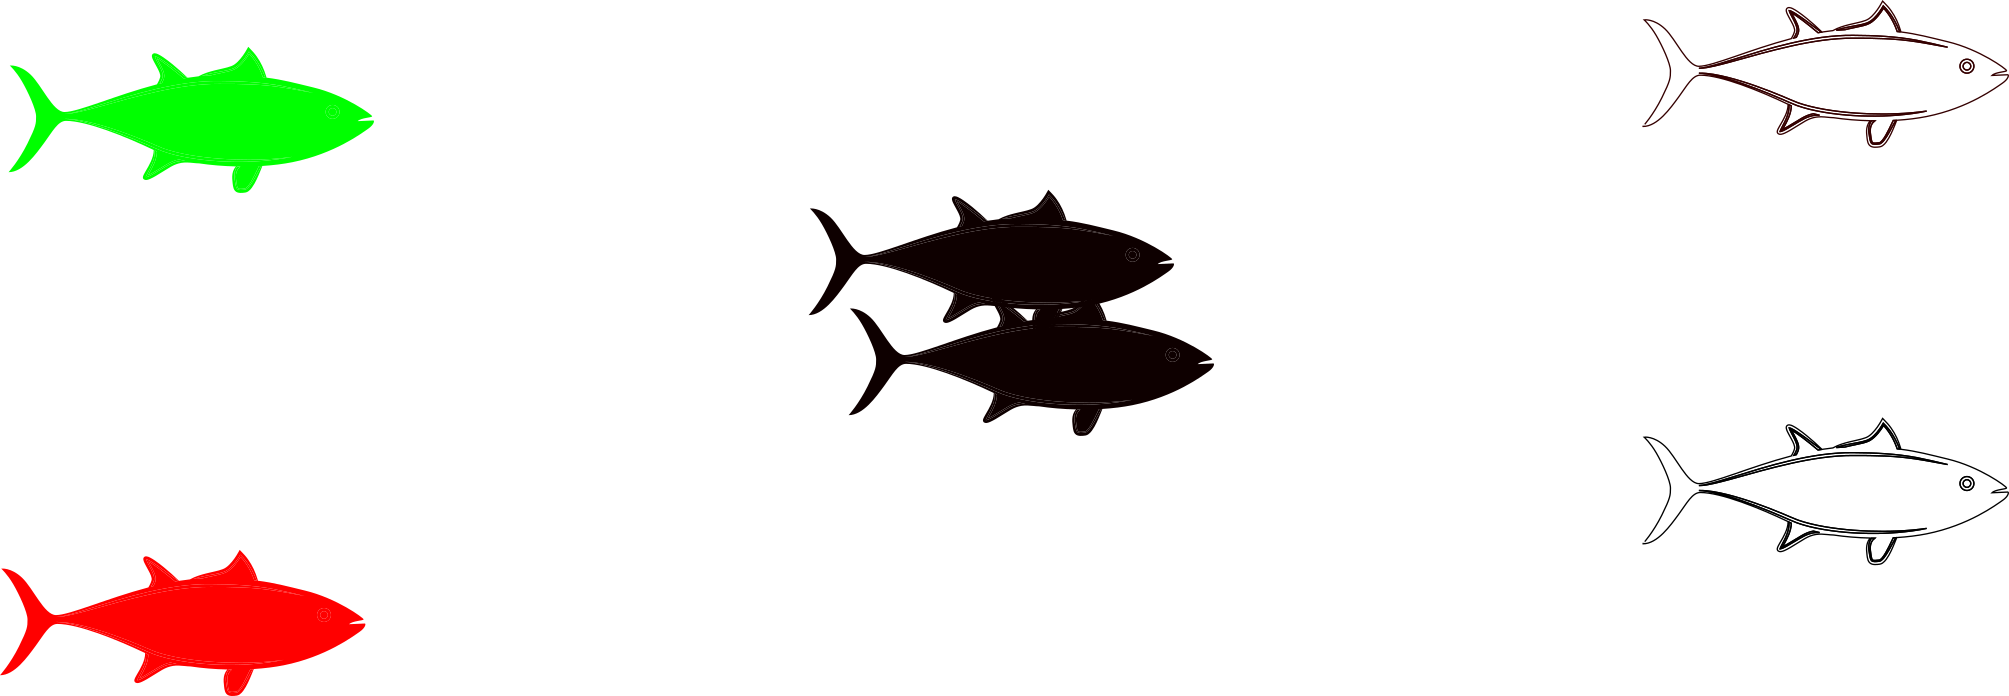
\includegraphics[width=\linewidth]{g1225}
%	\caption{The program doesn't respect continuity}
%	\label{fig:continuity}
%\end{figure}

%The issues can occur in two scenarios, where the fish get close enough that the program returns their only being one fish (figure~\ref{fig:overlap}), and when the fish move fast enough that they are closer to the other's previous position then their previous position. The first of these issues is the easier of the two to check, since it is fairly trivial to check for regions in which only one fish is reported (please see Appendix~\ref{appendix1}). While it is easy enough to check for the first of these issues, the second is a little tougher. To check for errors in these cases, the distance of each fish from its previous position must be compared to the distance from each fish to the other fishes previous position (Appendix~\ref{app:swapStatus}). If the software mistakes the positions of the fish, which we will refer to as a swap, it will look like the fish traveled longer than it should have.

% [This may be better in the results section.]
%What this leads to is issues in the end results, since they are in no way accurate due to this massive source of error. To fix this issue, we are applying two approaches in tandem, both a more common naive technique that tends to fail in areas where the fish are close together but is computationally light and works well when the fish are far apart; and a second one of comparing a unique identifier for each fish from moment to moment to find the fish with the same identifier which is much more accurate, but computationally intensive, which we got from the paper on the idTracker program from when they tried to tackle the same problem\cite{perez-escudero_idtracker_2014}. The reason we are using two processes to track the fish is that a common issue of the more common and simpler first method of automatic tracking is that whenever the position of the fish have been confused, the tracker has no way to regain the fishes' position and track which fish is which. To solve this issue, we need a way to track the fish from moment to moment in the cases where this common approach fails, which leads us to the second method.



\section{Methods}

\subsection{Video Collection}
While any actual experimentation on the fish is beyond the scope of this thesis, it is still useful to describe the process of gathering data. The basic setup of the labs we are taking data from is a tank with two fishes in it and a camera trained on them, as seen below. 
This setup produces a video for us to use, of which an example frame is shown below.


\begin{figure}[H]
	\centering
	\setlength{\mylen}{0.35\linewidth}
	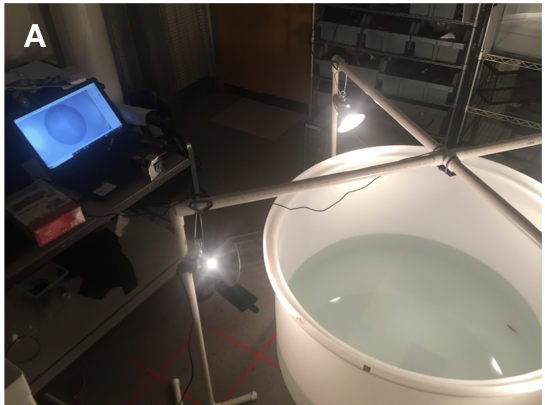
\includegraphics[height=\mylen]{experimental_design}
	\hspace{0.01\linewidth}
	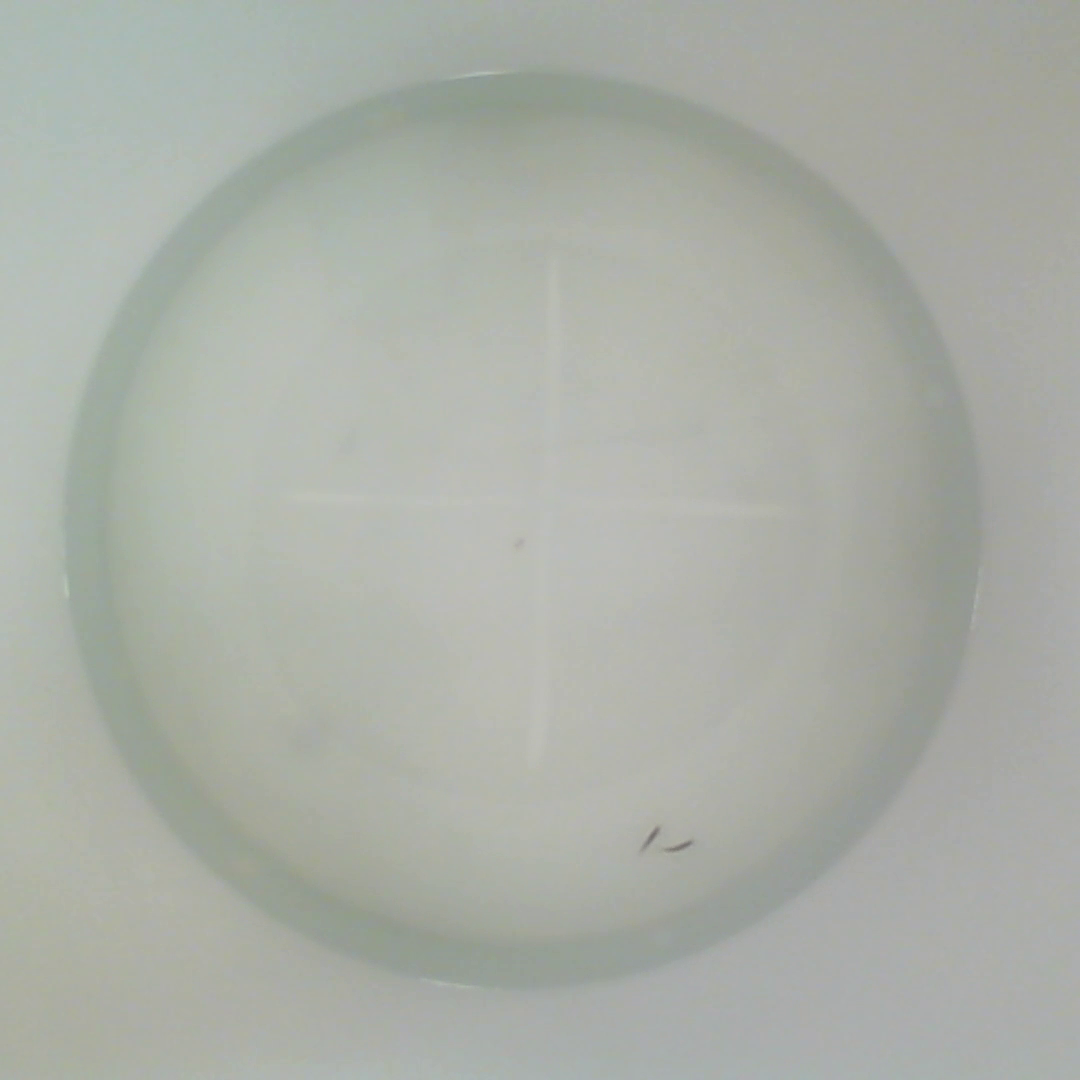
\includegraphics[height=\mylen]{figures.frame5140}
	\caption{\emph{Left}: The tank setup. \emph{Right}: An example frame of the video.}
\end{figure}


\subsection{Current Tracking}
%following is over explained
%say focusing on two fish somewhere
%expand this section

To track the fish, we must first feed the video captured from this setup to an analysis program, in our case cvtracer~\cite{patch_kinematic_2020, patch_patchmemorycvtracer_2020}, which has been especially created for use by the Jupiter Trilab. 
The tracker works taking the tank as a constant background, and noting that the fish are the only dark spots on the tank. It then returns an array for each of the fish containing a list of the fish's pixels and those pixel's colors. Once we have the fish saved in a format that we can analyze, we are ready to start working on the tracking of the fish. Since each the way we store the data gives each fish an identifier, we then can use those identifiers to analyse the fish.

%The next step is to segment the data into regions based on the number of fish it detects. We do this because the distance based unswapping approach doesn't work on regions where there is only one fish detected, so we need to tell the program where it can use that approach.
%
%\begin{figure}[H]
%	\centering
%	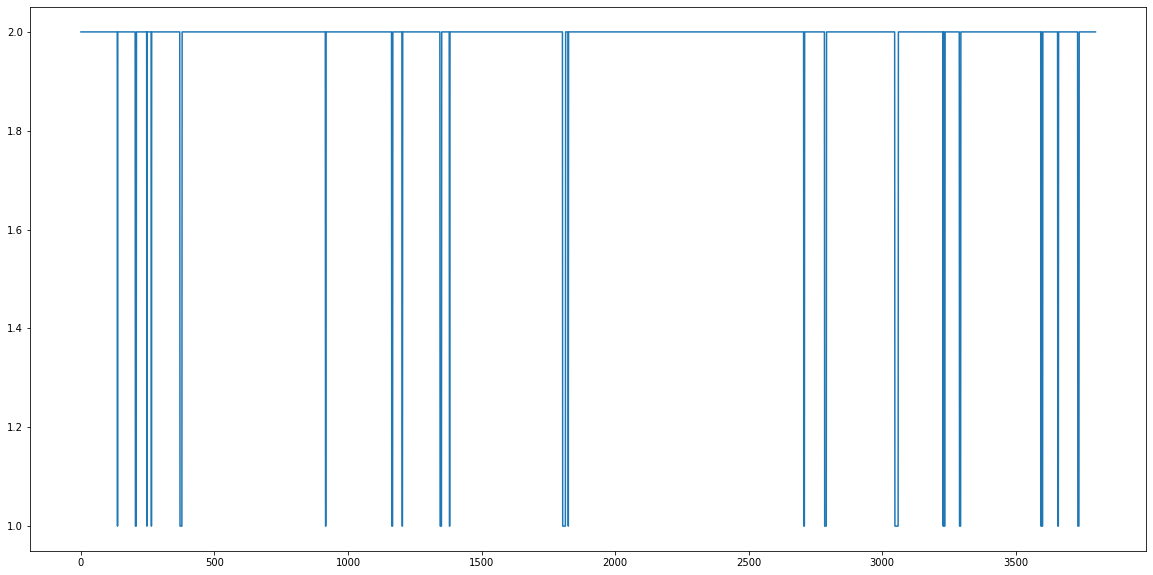
\includegraphics[width=.75\linewidth]{oneFish}
%	\caption{Number of one fish regions}
%\end{figure}


\subsection{Distance Based Unswapping}

The first and simplest round of identity unswapping works by minimizing the total distance traveled by the fish between the previous frame and the current one. Figure~\ref{fig:distance-unswap-principle} illustrates the way the method works for two fish. The semi-transparent fish indicate each fish's position in the previous frame. In the left panel, identities are maintained, and the distances traveled (double arrows) are small. In the right panel, an identity swap has occurred: in the new frame, the red fish has become blue and vice versa. Because of this swap, each fish appears to have traveled much more distance (double arrows) than it actually has.

\begin{figure}[H]
	\centering
	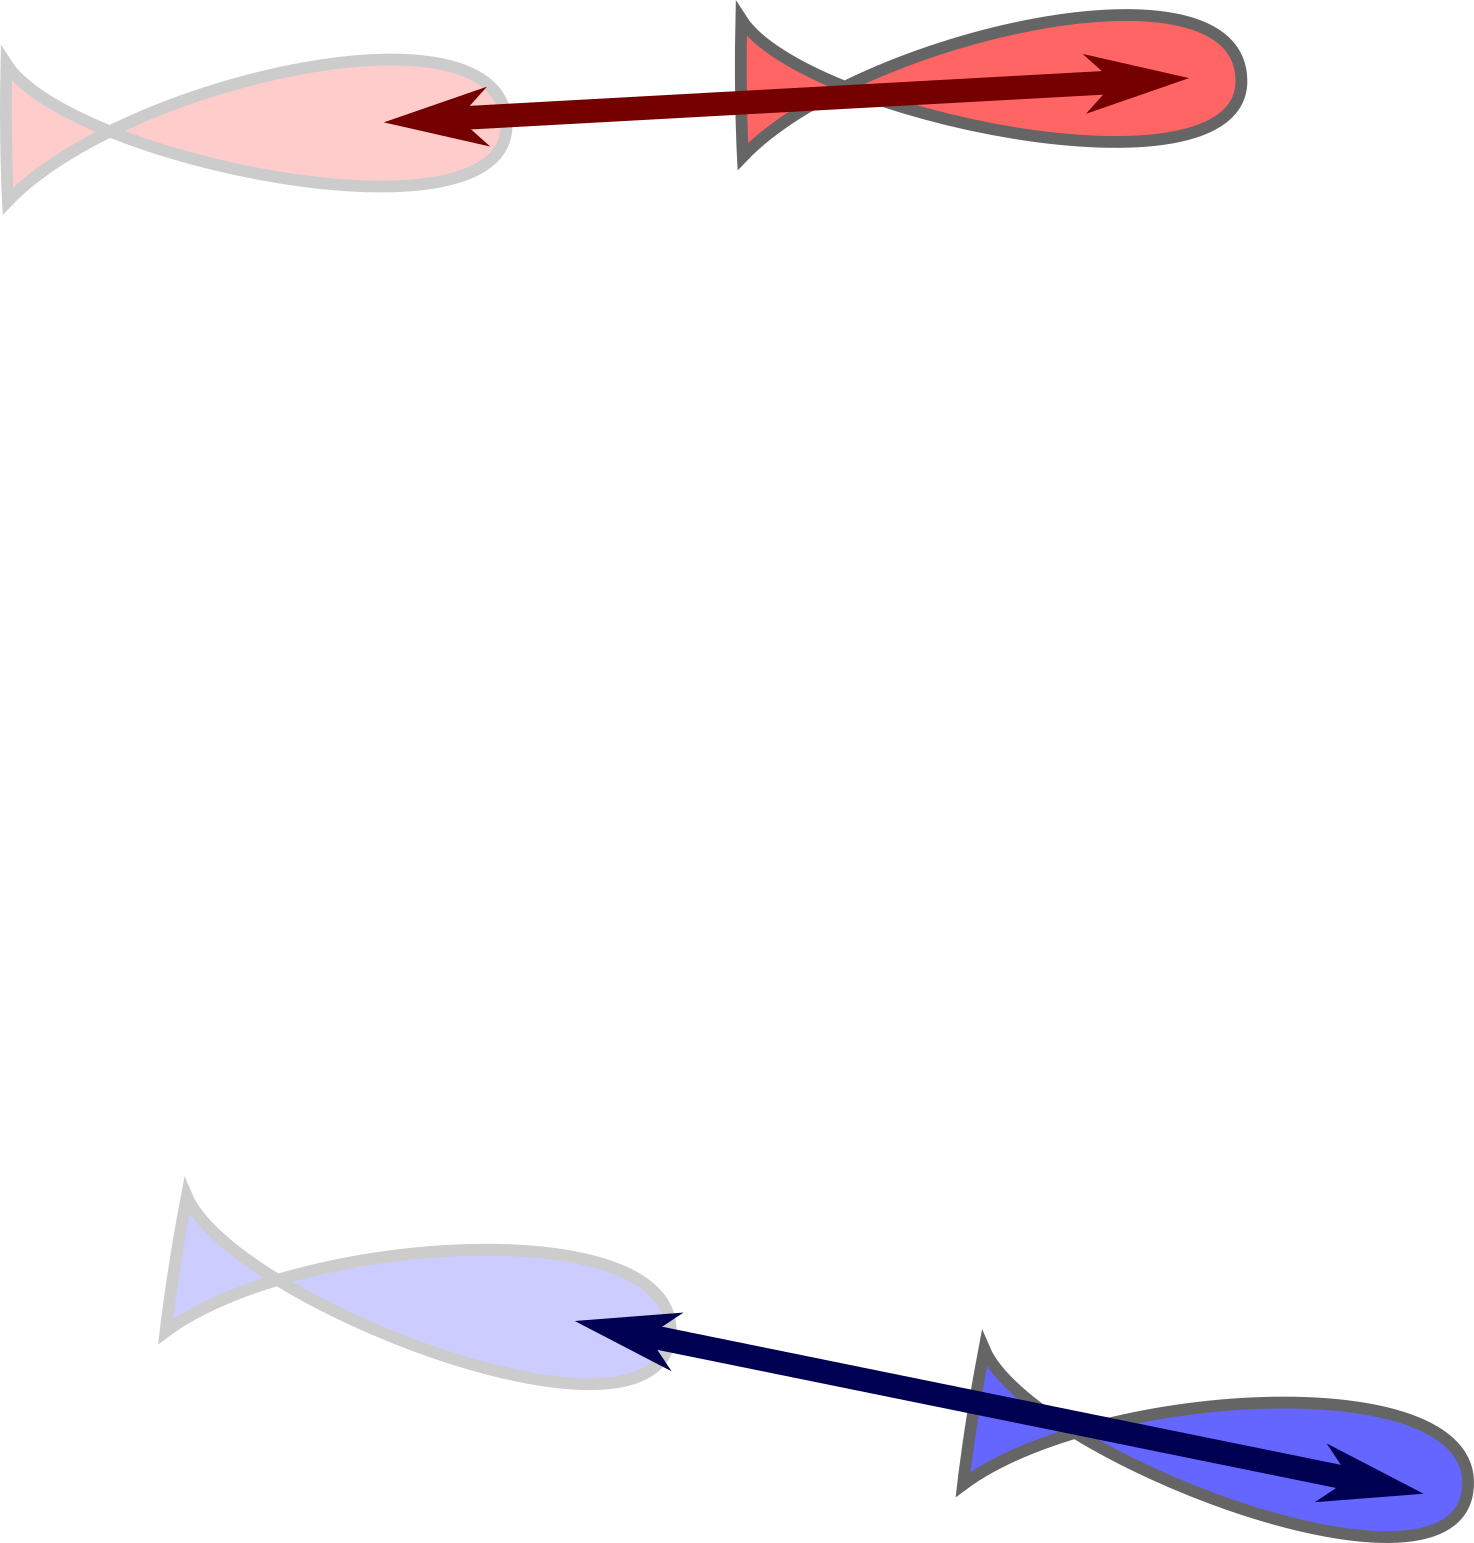
\includegraphics[width=0.4\linewidth]{distance-swap1}
	\hspace{0.05\linewidth}
	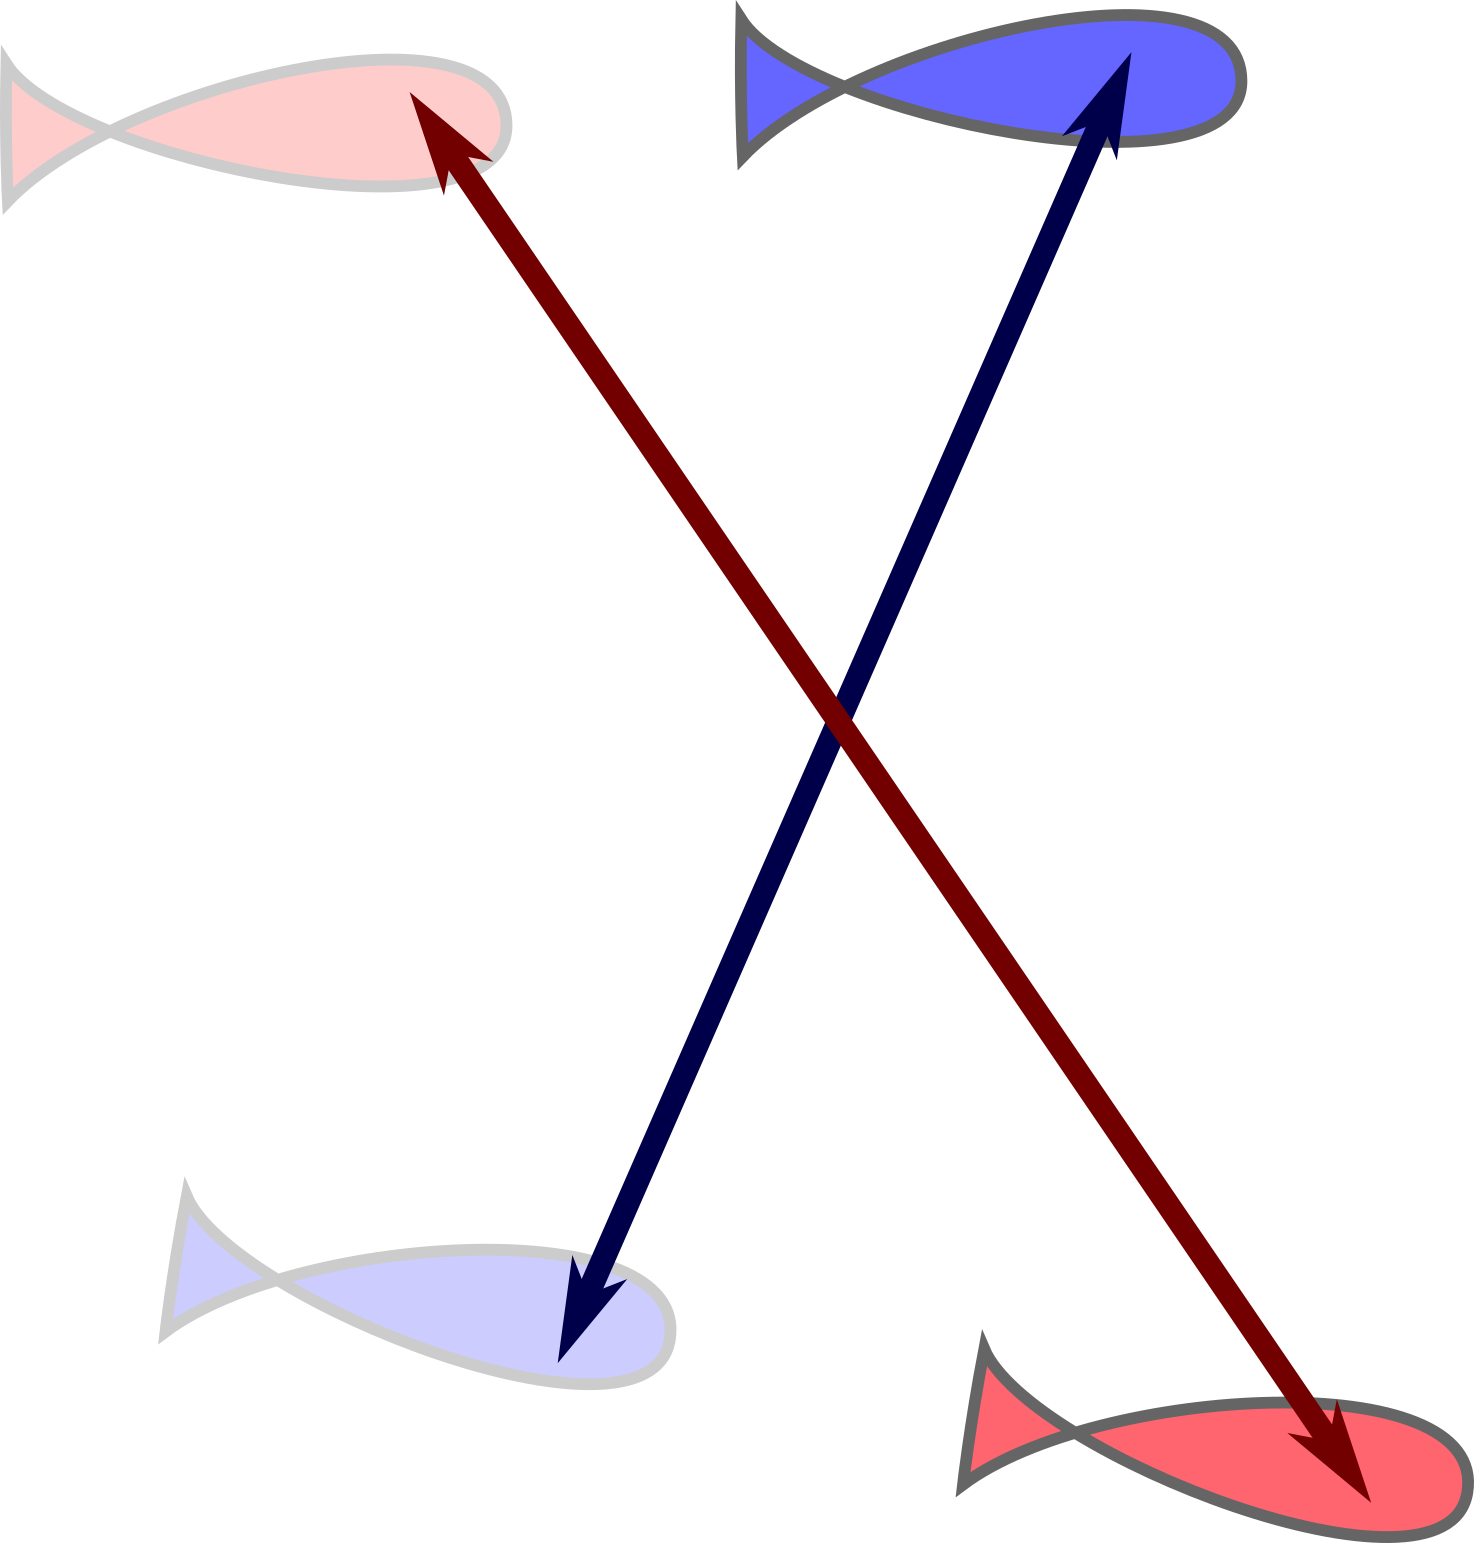
\includegraphics[width=0.4\linewidth]{distance-swap2}
	%	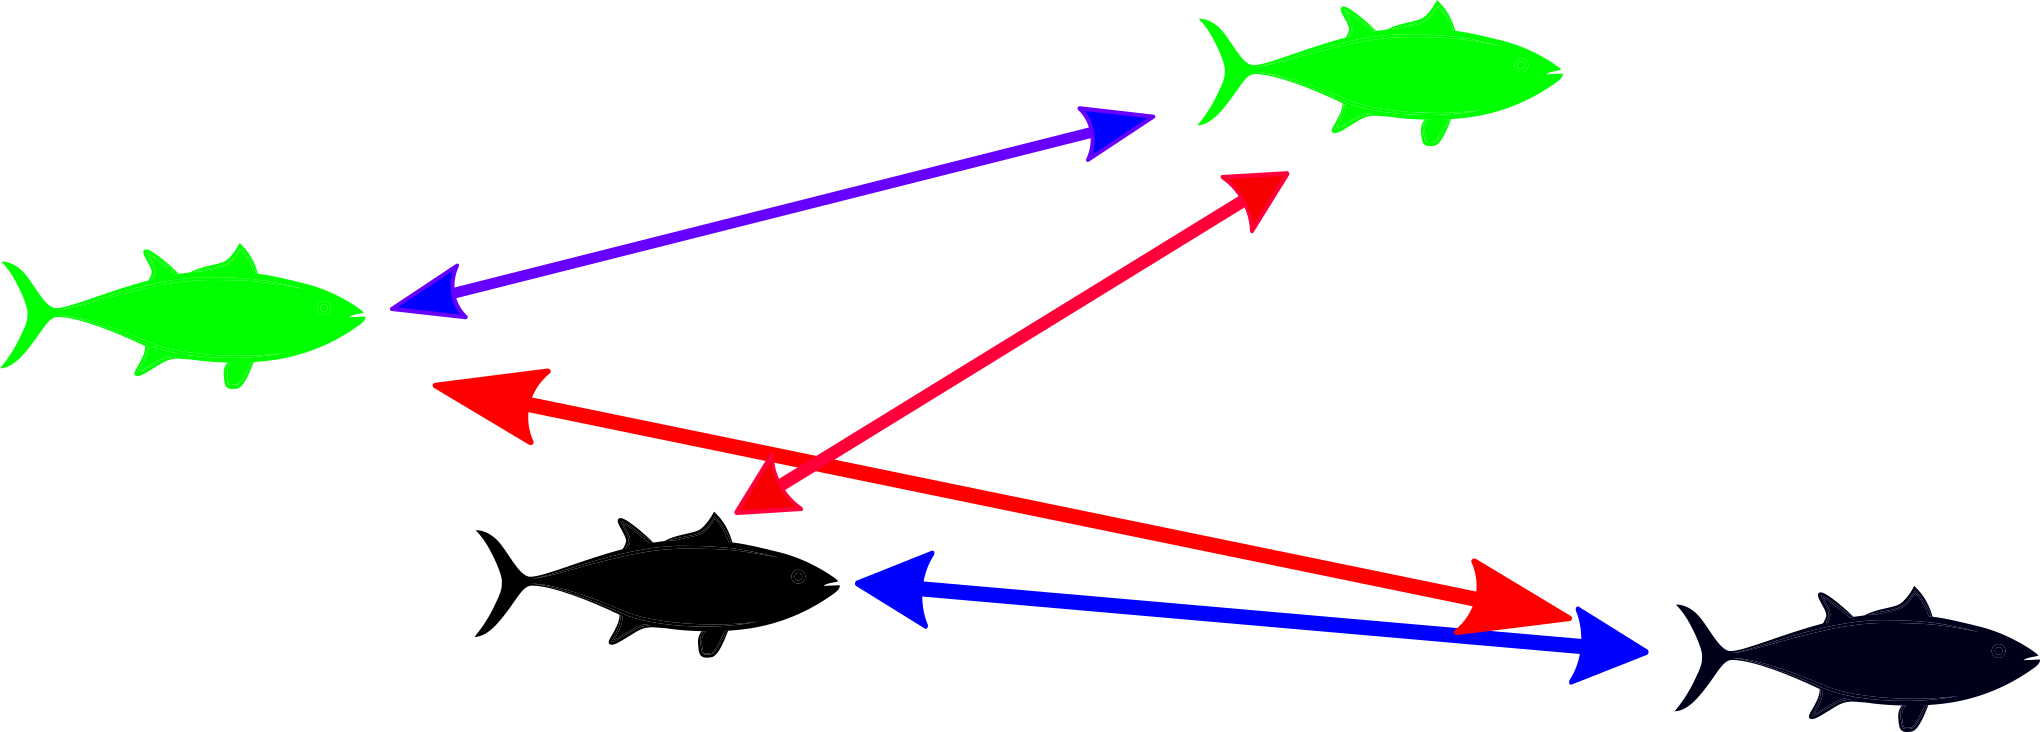
\includegraphics[width=.49\linewidth]{fish3}
	%	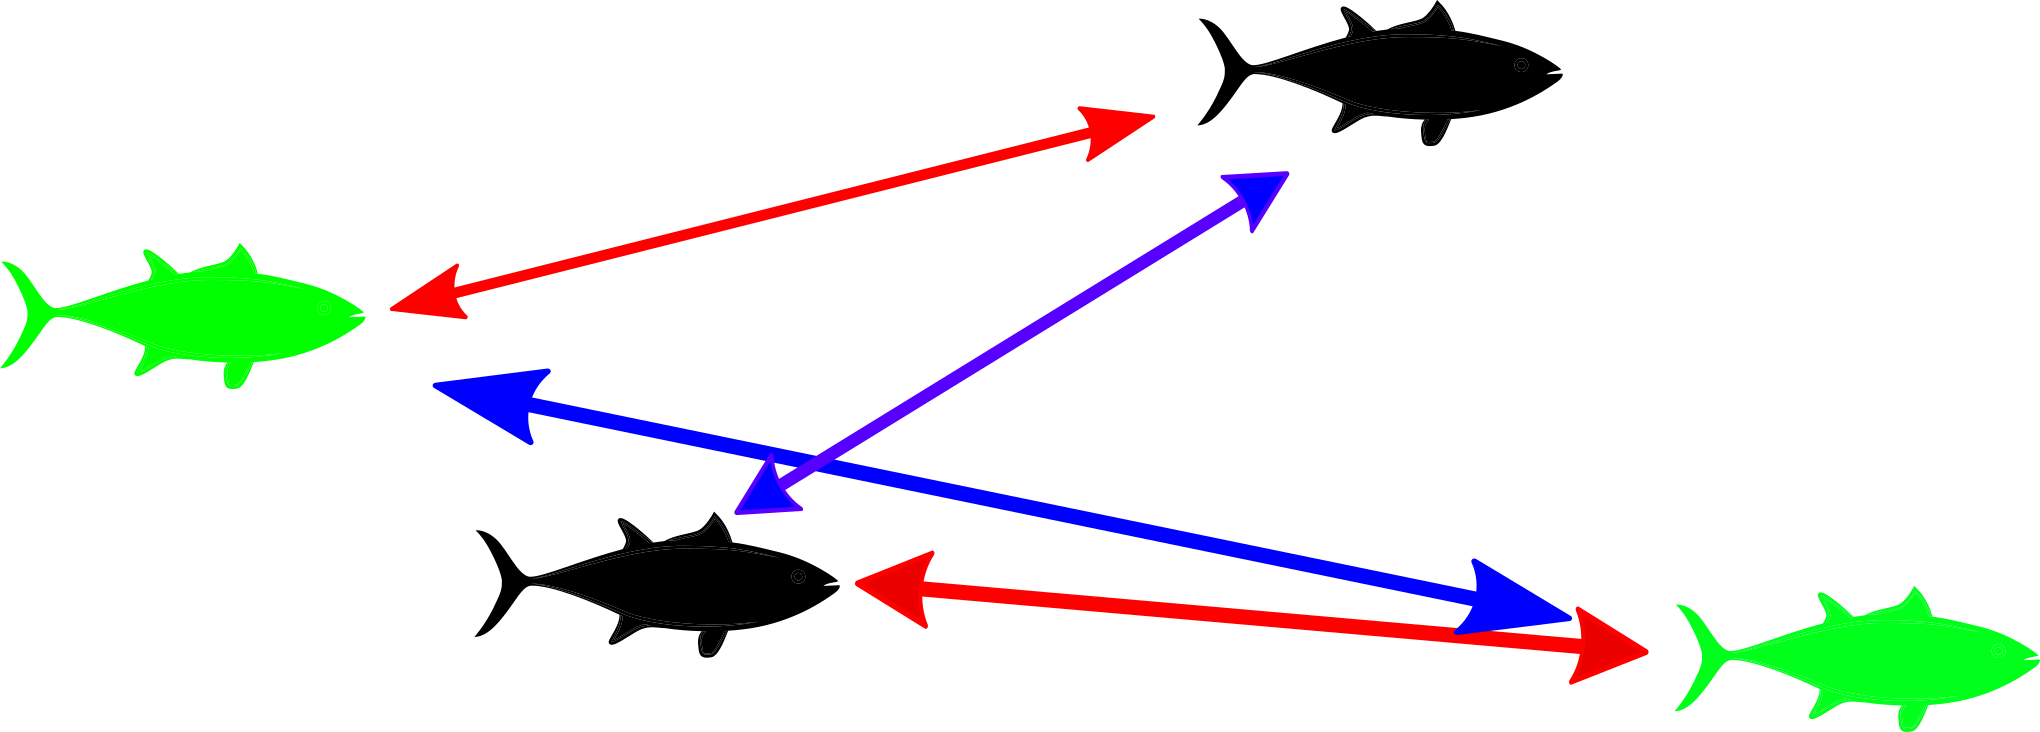
\includegraphics[width=.49\linewidth]{fish4}
	\caption{Distance traveled by the fish between two frames when identities are maintained (left panel) and when identities are swapped (right panel).}
	\label{fig:distance-unswap-principle}
\end{figure}

In order to determine whether a swap has occurred, we compute the following distance matrix, which contains all four of the distances shown in the figure:
%
\newcommand{\myMatrixItem}[1]{\begin{minipage}[b]{15em}\singlespacing{#1}\end{minipage}}
\begin{equation}
	\begin{pmatrix}
		\text{\myMatrixItem{distance from fish 1 in previous \\ frame to fish 1 in current frame}} 
			& \text{\myMatrixItem{distance from fish 1 in previous \\ frame to fish 2 in current frame}} 
		\\
		\text{\myMatrixItem{distance from fish 2 in previous \\ frame to fish 1 in current frame}} 
			& \text{\myMatrixItem{distance from fish 2 in previous \\ frame to fish 2 in current frame}} 
	\end{pmatrix}
	\nonumber
\end{equation} 
%
The sum of the diagonal terms (previous-1-to-current-1 and previous-2-to-current-2) represents the total distance traveled by both fish since the previous frame assuming identities were maintained. The sum of the two off-diagonal terms (previous-1-to-current-2 and previous-2-to-current-1) represents the total distance traveled by both fish since the previous frame assuming identities were swapped. If the latter is smaller than the former, then we conclude the identities were swapped.


%\begin{figure}[H]
%	\centering
%	\includegraphics[width=.75\linewidth]{fish2}
%	\caption{Basic overview of unswapping logic}
%\end{figure}


\subsection{Identifying overlaps}


\yf{[YF] Stopping here for now. After this I would first discuss the principle of the histogram method in a frame-to-frame context. Then, possibly in a separate methods subsection, discuss locating the overlaps and averaging the histograms over nonoverlapping ranges for a more accurate/less noisy comparison.}

\vspace{1in}

%The default method that the program uses to determine which fish is which is to assume that the fish closest to their previous positions are the same fish. However, this tends to fail in areas in which either the fish have moved a great distance since the last frame, or the case in which the fish are close enough that the program returns their only being one fish, in which case the program will basically assume which fish is which at random. To combat this we will use several methods. The first of these is distance based unswapping, which works by 

The first approach we tried is taking the positions of the fish and comparing how close they were to their previous positions to check for swaps. This approach works on the regions where there are two fish detected (``nonoverlapping range''), and so we need to confine it to those regions. 

\subsection{Histogram Based Unswapping}

Since the distance based approach works in regions where two fish are detected, a second approach is needed for one fish regions. The approach that we decided to work with for these sections was to take a identifier that was unique to each fish, and compare them against each other on a frame by frame basis. The identifier that we chose was the histogram created by taking the brightness of each fish (Appendix~\ref{app:histCreator}), as proposed by idTracker\cite{perez-escudero_idtracker_2014}, which has the advantage of being both one of the most unique things that it is possible to analyze about the fish and being easy to compare given that we can take the euclidean distance between histograms. To create these histograms, we are using numpy's histogram2d, which is ideal for our use case since it can be used directly without any other setup on our part besides determining bins, which we will do later in section~\ref{sec:binReduce}.

\begin{figure}[H]
	\centering
	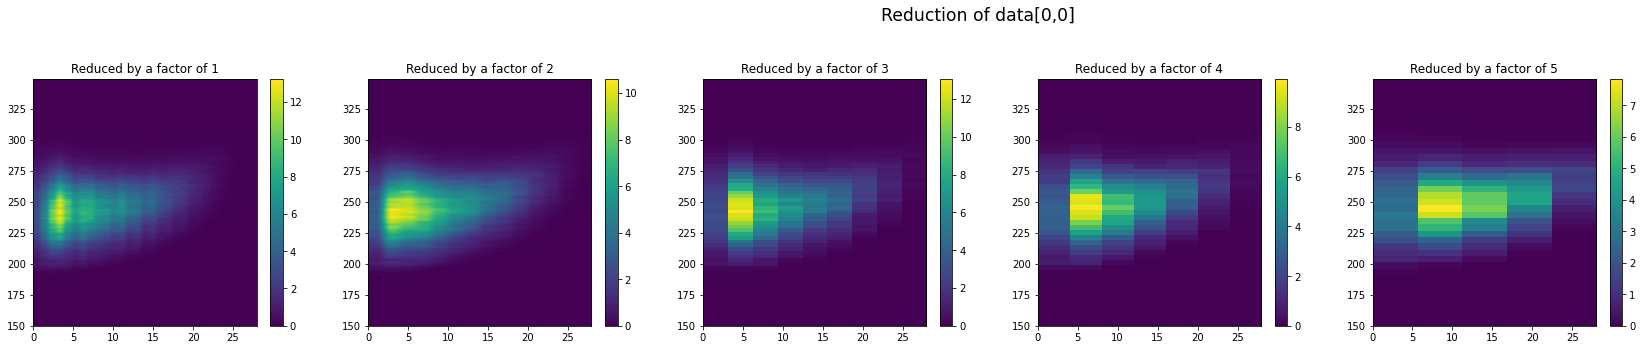
\includegraphics[width=\linewidth]{reducedHist}
	\caption{The histograms}
	\label{fig:reducedHist}
\end{figure}

\subsection{Averaging Overlaps}

One thing that we did to reduce variability in our answers was to average the regions over which the histograms were taken. By taking the histograms at the beginning and end of the overlapping range, we are able to both 

\section{Results}

\subsection{Accuracy}
%\textbf{\textit{show pictures and describe accuracy.}}

Without any tuning, the accuracy rate is only 19\%. This is probably due to the fish being too uniform, as once are able to tune the process, we can expect a slightly more accurate result.

\begin{figure}[H]
	\centering
	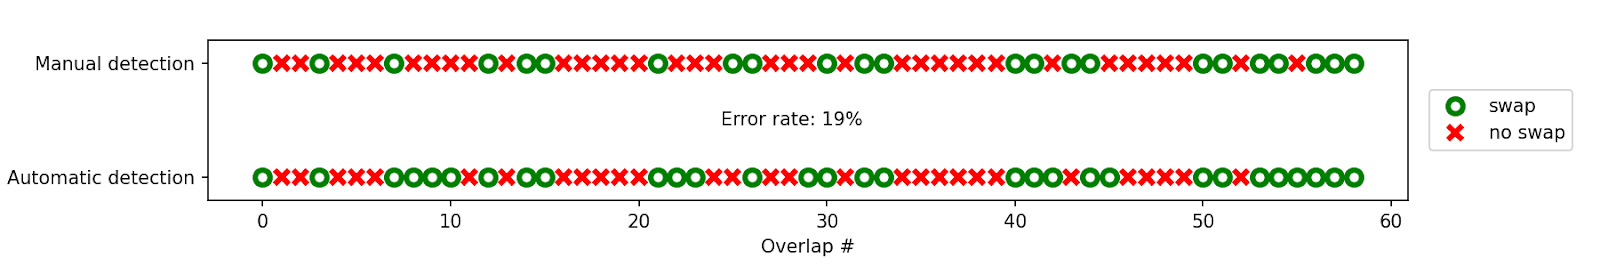
\includegraphics[width=\linewidth]{error}
	\caption{The error of the untuned process}
\end{figure}

\subsection{Bin Reduction}
\label{sec:binReduce}

One thing that was also tested was what would happen if we used less bins on the histograms that we used for analysis, both to see how it affected accuracy and performance. What was found was that there was no significant change in the accuracy of the data when this operation was performed. The most difference in accuracy that we were able to observe was 13\%, with that being an outlier considering most reductions were under 9\%, with the vast majority being under 6\%. 

\section{Code?}

After that we need to manipulate the data slightly so that the histograms are taken as the average over the nonoverlapping regions for more accuracy, and are then saved out for comparison. We can then feed this representation into a simple value comparison to check for swaps. When rendered to a more human readable form, we can either get a list of frames, or a graphs as shown below.

\begin{figure}[H]
	\centering
	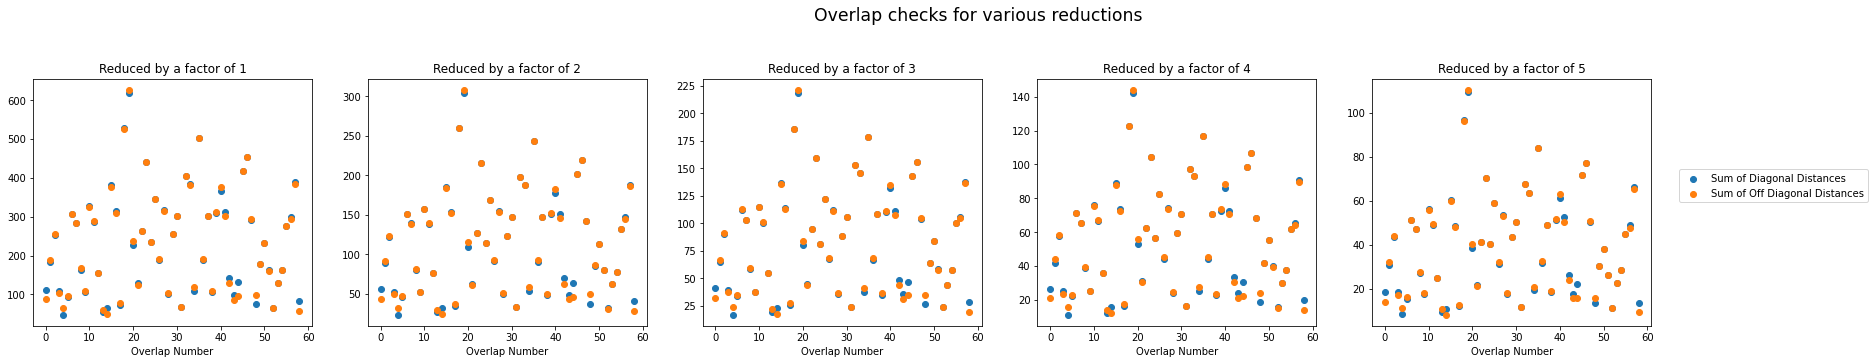
\includegraphics[width=\linewidth]{reducedGraph}
	\caption{The graphs from the histograms}
	\label{fig:reducedGraph}
\end{figure}


\appendix
\section{Appendix A}
\label{appendix1}

\begin{minipage}[c]{\textwidth}
\begin{lstlisting}[language=Python]
i2=0
nonOverlappingRange=[]
while i2<len(fish):
    i1=i2
    while i1<len(fish) and len(fish[i1])!=2:
        i1+=1
    i2=i1
    while i2 < len(fish) and len(fish[i2])==2:
        #find the first overlapping index
        i2+=1
    nonOverlappingRange.append([i1,i2])
print(nonOverlappingRange)
\end{lstlisting}
\end{minipage}

\section{Appendix B}
\label{app:swapStatus}

\begin{minipage}[c]{\textwidth}
\begin{lstlisting}[language=Python]
def swapStatus(pos,i):
    '''
    Detect swaps between consecutive frames based on proximity.
    
    Input:
        pos:Postionts. Array with shape (Nframes,Nfish,Ndimensions),
        i: Frame index. Int.
    
    Output:
        Int. 0 if no swaps, 1 if swapped, 2 if overlapping.
    '''
    nFish=pos.shape[1] #Number of fish
    distanceMatrix=[np.linalg.norm(pos[i+1][0]-pos[i][0]),
                    np.linalg.norm(pos[i+1][1]-pos[i][1]),
                    np.linalg.norm(pos[i+1][0]-pos[i][1]),
                    np.linalg.norm(pos[i+1][1]-pos[i][0])]
    swapCriteron=(distanceMatrix[0]+distanceMatrix[1])-(distanceMatrix[2]+distanceMatrix[3])
    if abs(swapCriteron)<1e-10:
        return 2 #Overlapping
    elif swapCriteron>0:
        return 1 #Swapped
    elif swapCriteron<0:
        return 0 #Normal
    else:
        return -1
\end{lstlisting}
\end{minipage}

\section{Appendix C}
\label{app:dataShape}

The data is stored in an array of shape [frame][fish][xpixels,ypixels][color]

\textit{\textbf{Picture Here}}

\section{Appendix D}
\label{app:histCreator}

\begin{minipage}[c]{\textwidth}
\begin{lstlisting}[language=Python]
for i in tnrange(60,desc='nonOverlappingRange'):
    for k in range(2):
        countSum=0
        countDif=0
        pairData=[]
        for j in range(*nonOverlappingRange[i]):
            fishPixels = fishU[j][k]
            m,l=np.triu_indices(fishPixels.shape[0],k=1)
            d=np.sqrt((fishPixels[l,0]-fishPixels[m,0])**2+(fishPixels[l,1]-fishPixels[m,1])**2)
            bSum=fishPixels[l,2]+fishPixels[m,2]
            bDif=fishPixels[l,2]-fishPixels[m,2]

            heightValuesSum,_,_=np.histogram2d(d,bSum,bins=(binsDist,binsSum))
            histSum+=heightValuesSum
            countSum+=1
            heightValuesDif,_,_=np.histogram2d(d,bDif,bins=(binsDist,binsDif))
            histDif+=heightValuesDif
            countDif+=1
        histSum/=countSum
        histSumList[i,k]=histSum.copy()
        histDif/=countDif
        histDifList[i,k]=histDif.copy()
\end{lstlisting}
\end{minipage}

%==========================================================================
% Bibliography.

\bibliographystyle{plain}
\bibliography{fish}


\end{document}
